\chapter{Постановка задачи}\label{ch:ch1}
\section{Обзор робота}\label{sec:ch1/sec1}
В данной задаче используется робот, собранный из сервомоторов Kondo,  неподвижных частей, с оборудованием для ориентации робота в пространстве: акселерометр, гироскоп, магнитометр (рисунок ~\cref{fig:real_robot}). Каждый сервомотор обеспечивает поворот вдоль заданной оси в заданном интервале углов. Движение может происходить как по часовой стрелке, так и против. Для каждого мотора задаётся свой интервал углов, чтобы избегать повреждения робота вследствие самопересечения конструкции робота. В итоге 23 сервомотора задают 23 степени свободы движений робота. Так как мы исследуем возможности ходьбы, то ограничимся только на 12 сервомоторов – по 6 для каждой ноги (рисунок ~\cref{fig:sim_robot_2-1})

\begin{figure}[ht]
    \centerfloat{
        \label{fig:real_robot-1}}{%
            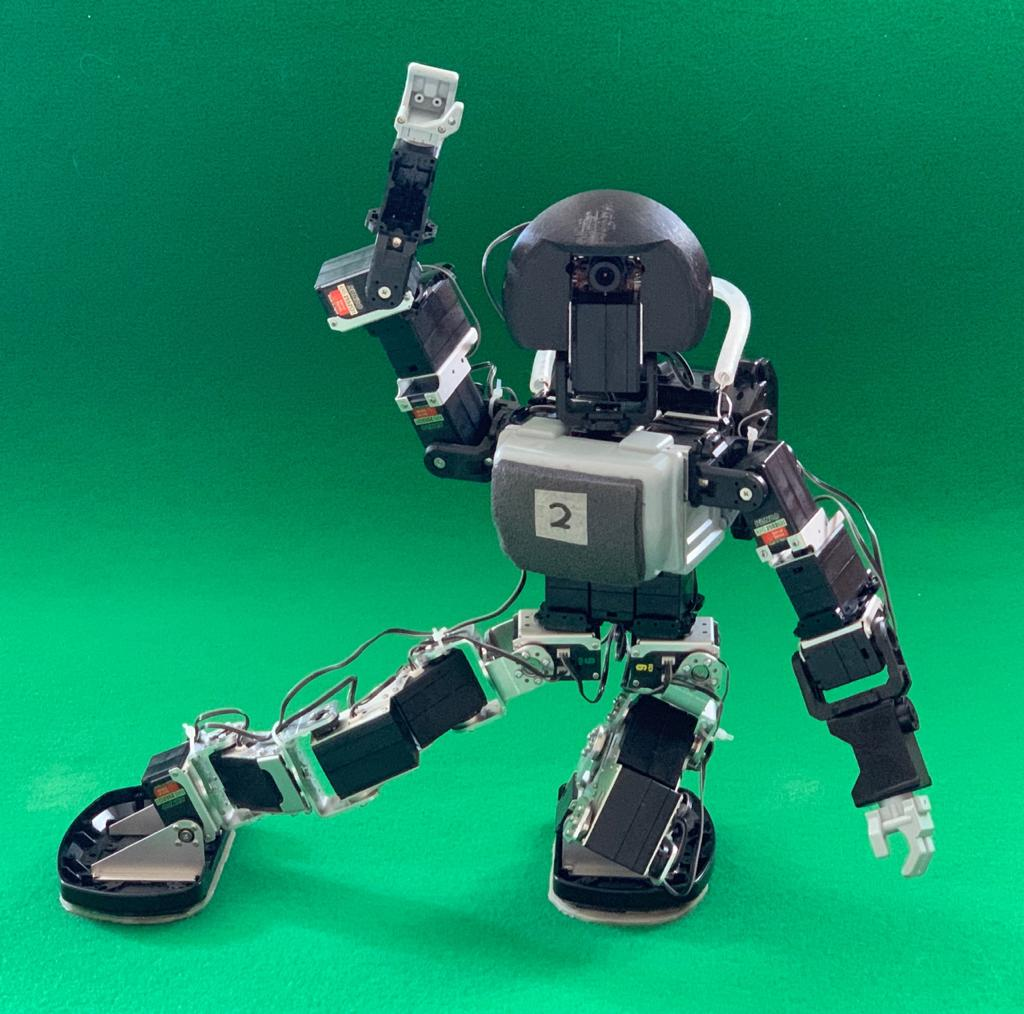
\includegraphics[width=0.5\linewidth]{real_robot}}
    \caption[Изображение робота в действии]{Изображение робота в действии}\label{fig:real_robot}
\end{figure}
\section{Используемый симулятор}\label{sec:ch1/sec1}

Для ускорения исследования используется симулятор CoppeliaSim \cite{coppeliaSim} Работа в симуляторе позволяет производить параллельные вычисления, а также модифицировать параметры окружающей среды: изменять рельеф, добавлять препятствия и создавать толкающие усилия в направлении робота. 

В симуляторе представлена (рисунок ~\cref{fig:sim_robot_2-2}) упрощённая модель робота. Модель состоит из примитивных объектов: сфера, параллелепипед и цилиндрический сервомотор. Это позволяет значительно ускорить вычисления, при этом наследуются все важные для ходьбы физические свойства реальной модели.

\begin{figure}[ht]
    \centerfloat{
        \hfill
        \subcaptionbox[List-of-Figures entry]{Модель робота целиком\label{fig:sim_robot_2-1}}{%
            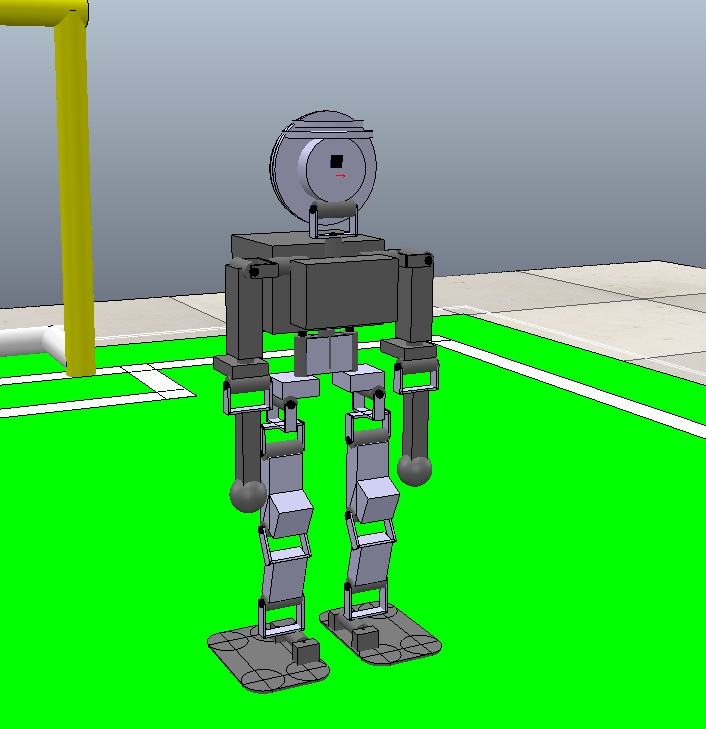
\includegraphics[width=0.4\linewidth]{sim_robot}}
        \hfill
        \subcaptionbox{Сервомоторы ноги \label{fig:sim_robot_2-2}}{%
            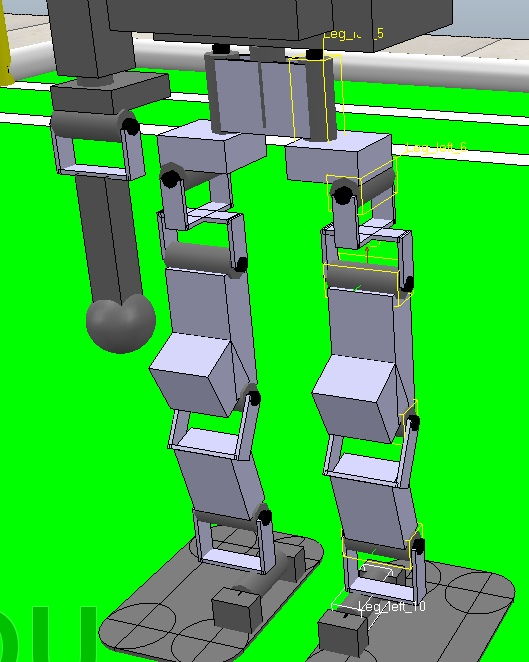
\includegraphics[width=0.328\linewidth]{foot}}
        \hfill
    }
    \caption[Обзор модели робота в~симуляции]{Обзор модели робота в~симуляции}\label{fig:sim_robot_2}
\end{figure}

Взаимодействие с симулятором будет осуществляться через проект PyRep \cite{james2019pyrep} Преимущество этого подхода в том, что нет затрат времени на межпроцессорное взаимодействия программы обучения и симулятора, есть возможность запускать несколько симуляций параллельно.

\section{Определение марковского процесса принятия решений}\label{sec:ch1/sec3}
Одним из подходов описания процесса взаимодействия управляющей программы со средой является марковский процесс принятния решения. Процесс задаётся четвёркой $\left<S, A, T, R\right>$, где $S$~--- множество состояний среды, $A$~--- множество возможных действий управляющей программы. $T: S\times A \times S \rightarrow [0, +\inf)$ определяет распределение вероятности на множестве $S$, иначе говоря $\forall s, s' \in S,\ a\in A:\ T(s, a, s') = P(s' | s, a)$. Функция $R : S \times A \ \times S \rightarrow \mathbb{R}$ определяет награду, которую получает агент (управляющая программа), например, если, выполнив действие $a$, был осуществлён переход и состояния $s$ в состояние $s'$, то агент получается за этот ход награду, равную $R(s, a, s')$. 

Для возможности выполнения алгоритма непрерывное время в среде дискретизируется. А именно каждые $\tau$ миллисекунд состояние $s_t \in S$ меняется на $s_{t+\tau} \in S$ после выполнения действия $a \in A$.

В действительности вероятности переходов $T$ не изветсны, но можно описать множество событий и множество действий, а также награду и цель агента.

\subsection{Множество состояний $S$}
Так как каждая нога робота имеет по 6 степеней свободы, то вектор $\theta \in {[0, 1]}^{12}$ задаёт углы поворота каждого мотора ног относительно минимального и максимального допустимых значний. А также благодаря датчикам в роботе мы можем восстановить его ориентацию относительно земли, получив трёхмерный вектор $v\in \mathbb{R}^3, ||v|| = 1 $. А значит $S = \left\{    \begin{pmatrix}
        \theta\\
        v
    \end{pmatrix}| \theta \in {[0, 1]}^{12}, v\in \mathbb{R}^3, ||v|| = 1\right\}$. Здесь производится основное предположение, что этот вектор однозначно задаёт робота в пространстве, поэтому мы можем говорить о марковом процессе.

\subsection{Множество действий $A$}
Действием агента назовём целевые положения моторов на следующем цикле исполнения среды, а значит $A = {[0, 1]}^{12}$.

\subsection{Определение функции награды $R$}
Выбрать подходящую функцию награды~---  трудная задача. Обычно она решается в ходе экспериментов методом проб и ошибок. Но на текущем этапе можно сформулировать её вид: $l_2$ норма отклонения вектора скорости центра масс робота $v_{zmp}$ от желаемого ускорения $v_{target}$.

Обычно функция награды является частью среды, поэтому можно считать, что для её расчёта доступна дополнительная информация помимо пространства событиый $S$.

\subsection{Цель агента}

Цель агента~--- максимизация дисконтированной суммы наград:

$$
\sum\limits_{i}^{i < k} \gamma ^{k - 1 - i} R(s_{i \cdot \tau}, a_{i \cdot \tau}, s_{(i+1) \cdot \tau})
$$

Где $\gamma \in [0, 1]$~--- параметр дисконтированния, а $k$~--- количество циклов с начала симуляции. 